\chapter{Stochastic Switching Linear Control using Nonlinear Hybrid Models}
\label{sec_spf_control}
We continue our discussion of switching control from Chapter \ref{sec_rbpf_control} here. In this section we use the Switching Particle Filter to identify the best model to use in the stochastic controllers we developed in Chapter \ref{sec_linear_control}. More precisely, let $M_i = (A_i, B_i)$ be the linearised model of the nonlinear models $(f_i, g_i)$ as discussed in Chapter \ref{sec_inf_spf}. By using the most likely model resulting from the Switching Particle Filter we aim to design a controller which is robust against system faults.

We assume the same scenario as introduced in Chapter \ref{sec_spf_filtering} i.e. we assume we have 2 nonlinear plant models available. Model $M_1$ corresponds to the healthy CSTR and model $M_2$ corresponds to the CSTR with denatured catalyst (the faulty model). We will again avail ourselves of the Switching Controller Algorithm  repeated here for convenience.

\textbf{Switching Controller Algorithm}:
\begin{enumerate}
\item
Use a switching filter algorithm, e.g. the Switching Particle Filter, to update the state estimates of the particle population given the current observation. See Chapter \ref{sec_inf_spf} for more details.
\item
Select the particle with the highest switching weight. Since each particle corresponds to a certain model we implicitly have the most probable model $M_i$.
\item
Use the mean and covariance information encoded by this particle within the context of the stochastic controller (LQG or MPC) formulation of Chapter \ref{sec_linear_control}. Use the most likely model, $M_i$ from step 2, in this setting.
\item
Repeat for the next observation. 
\end{enumerate} 
Recalling Chapter \ref{sec_switch_mpc_lit} we note that it is possible to incorporate the model switching into the optimisation problem but at the cost of a significantly increased computational burden. Like Chapter \ref{sec_rbpf_control} we simplify the problem by only using a single model in the controller algorithm but we allow this model to change based on the system observations. A coincidental benefit of this approach is that the controller will automatically detect the modelled fault. 

Since the underlying Graphical Model in Chapter \ref{sec_inf_lin_hybrid} and Chapter \ref{sec_inf_spf} is the same, we expect the global trends to be the same as those found in Chapter \ref{sec_rbpf_control}. For the sake of illustration we exclusively use both state measurements. There is no fundamental reason why one cannot use only one state measurement except that the filter performance will be worse.

For the remainder of this section we assume the control goal is to keep the the system at the unsteady concentration operating point of the healthy model, even in the presence of the denatured catalyst.

\section{Unconstrained Switching Control}
\label{sec_spf_uncon}
In this section we compare the standard LQG controller (discussed in Chapter \ref{sec_lqg_lit} and \ref{sec_uncon_lin_control}) to the Switching Controller Algorithm implemented within the context of the LQG controller as shown in (\ref{eq_spf_lqg}). The same control parameters as those found in Chapter \ref{sec_lin_sys_cont} are used.
\begin{equation}
\begin{aligned}
&\underset{\mathbf{u}}{\text{min }} \mathbb{E}\left[ \frac{1}{2}\sum_{k=0}^{N-1} \left( x_k^TQx_k + u_k^TRu_k \right) + \frac{1}{2}x_N^TP_fx_N \right] \\
& \text{subject to } x_{t+1}=A_ix_t+B_iu_t + w_t~\text{(Latent)} \\
& \text{and } y_{t}= Cx_t + v_t \text{ (Observed)}\\
\end{aligned}
\label{eq_spf_lqg}
\end{equation}
Note that we select $M_i=(A_i, B_i)$ as the most likely model based on the switch weight at each time step. This model is then used in (\ref{eq_spf_lqg}) and solved using the techniques of Chapter \ref{sec_uncon_lin_control}
 
In Figure \ref{fig_spf_pf_lqg_track} we see the performance of the LQG controller applied to the CSTR system. At 100 minutes the catalyst denatures and the model used to design the controller becomes grossly inaccurate. The inappropriateness of the model also affects the Particle Filter's performance. 
\begin{figure}[H] 
\centering
\includegraphics[scale=0.25]{spf_pf_lqg_track.pdf}
\caption{Standard LQG controller applied to the CSTR where the catalyst denatures at 100 minutes. The bootstrap Particle Filter was used for inference and the Gaussian approximation of the particles was used.}
\label{fig_spf_pf_lqg_track}
\end{figure}
The average concentration error is 14.31\% and the average controller input is 120 kJ/min over the course of the simulation. We can clearly see that there is non-zero set point offset and control is bad in the sense of Definition \ref{def_stoch_ref_track_goal}. Clearly the standard LQG controller is ineffective in this scenario.

This motivates the use of a controller which intelligently changes the model control is based upon, as discussed previously. In Figure \ref{fig_spf_lqg_track} we see the set point tracking ability of the Switching Controller Algorithm using the LQG controller. Also note the superior filtering performance of the Switching Particle Filter.
\begin{figure}[H] 
\centering
\includegraphics[scale=0.25]{spf_lqg_track.pdf}
\caption{Switching LQG controller applied to the CSTR where the catalyst denatures at 100 minutes.}
\label{fig_spf_lqg_track}
\end{figure}
The average concentration error is 2.97\% and the average controller input is 129 kJ/min. It is clear that we have set point tracking even after the catalyst denatures. By inspecting Figure \ref{fig_spf_lqg_switch} we see that this is not surprising: the filter correctly identifies when the underlying model changes and then uses the better model for control. 
\begin{figure}[H] 
\centering
\includegraphics[scale=0.25]{spf_lqg_switch.pdf}
\caption{Most likely model identified using the Switching Particle Filter within the context of the Switching LQG Controller Algorithm.}
\label{fig_spf_lqg_switch}
\end{figure}
However, like in Chapter \ref{sec_rbpf_control_uncon} and \ref{sec_spf_filtering} we see that there is some switching noise. In Chapter \ref{sec_rbpf_control_uncon} this caused controller instability because the filter would switch between the different models too rapidly. Fortunately this is not the case here - the filter only briefly selects the working model $M_1$ when the system is in the regime of the faulty model $M_2$. The model oscillations are much less pronounced here.

The cause of this problem is that the models are too similar: the filter cannot clearly distinguish between them at all times. The problem would be exacerbated if only one state measurement was made. When we compared Figures \ref{fig_spf_m1_switch} and \ref{fig_spf_m2_switch} we saw that the additional measurement greatly benefited the filter's ability to discern between the models.

\section{Constrained Switching Control} 
In this section we extend the Switching Controller Algorithm of Chapter \ref{sec_spf_uncon} to the stochastic MPC introduced in Chapter \ref{sec_lin_mpc_constained}. We neglected implementing the stochastic MPC using the Rao-Blackwellised Particle Filter of Chapter \ref{sec_rbpf_control} because the switching noise (model selection) issues were too pronounced. We use the same parameters and measure both states. 

Like in Chapter \ref{sec_lin_sys_cont} we first illustrate the performance of the stochastic MPC controller with expected value constraints shown in (\ref{eq_spf_mpc_expected}) (for some model $M_i$) and then incorporate chance constraints later.
\begin{equation}
\begin{aligned}
&\underset{\mathbf{u}}{\text{min }} \mathbb{E}\left[ \frac{1}{2}\sum_{k=0}^{N-1} \left( x_k^TQx_k + u_k^TRu_k \right) + \frac{1}{2}x_N^TP_fx_N \right] \\
& \text{subject to } x_{t+1}=A_ix_t+B_iu_t + w_t~\text{(Latent)} \\
& \text{and } y_{t}= Cx_t + v_t \text{ (Observed)}\\
& \text{and } \mathbb{E}[\begin{pmatrix}
10 \\ 1
\end{pmatrix}^Tx_t + 400] \geq 0 ~\forall ~t=1,...,N \\
& \text{and } |u_t| \leq 15000 ~\forall ~t=0,...,N-1\\
\end{aligned}
\label{eq_spf_mpc_expected}
\end{equation} 
Using the results of Chapter \ref{sec_lin_mpc_constained} we know that (\ref{eq_spf_mpc_expected}) can be reformulated as a deterministic problem given the (Gaussian) state estimate $x_0$. The state estimate is derived from either the Particle Filter or Switching Particle Filter using 200 and 500 particles respectively.

In Figure \ref{fig_spf_pf_mpc_track} we see the set point tracking performance of the (\ref{eq_spf_mpc_expected}) using the same Particle Filter as used in Chapter \ref{sec_spf_uncon}. Since the Particle Filter only uses the healthy plant model we only use $M_1$. 
\begin{figure}[H] 
\centering
\includegraphics[scale=0.25]{spf_pf_mpc_track.pdf}
\caption{Deterministic MPC using a Particle Filter as the state estimator. The initial point is $(0.55, 450)$. An integrating disturbance model was used to estimate the mismatch between the underlying system and the controller model. The catalyst denatures at 100 minutes.}
\label{fig_spf_pf_mpc_track}
\end{figure}
Taking into account the discussion in Chapter \ref{sec_switch_mpc_lit} on zero offset\footnote{The results of this section implement the constant disturbance model to achieve zero set point offset. To keep notation the same we do not explicitly show it in (\ref{eq_spf_mpc_expected}) but mention it here.} MPC we expect the controller to be more effective than the corresponding LQG controller of Chapter \ref{sec_spf_uncon}. This is indeed the case. The average concentration error is 8.33\% and the average controller input is 145 kJ/min. 

Unfortunately we do not observe zero set point offset control but rather zero offset state estimates. Clearly the controller input generated by the MPC, which is based on the healthy plant, drives the Particle Filter's predictions to the set point. Note that the Particle Filter's model is only based on the healthy plant. We can see that the classic disturbance model approach \cite{lee} to ensure zero set point offset fails here because the underlying (faulty) model is too different from the controller model. Intuitively, we are attempting to control a tricycle (the faulty plant) using a model of a Ferrari.  

In Figure \ref{fig_spf_mpc_track} we see the Switching Controller Algorithm applied within the context of (\ref{eq_spf_mpc_expected}). The model corresponding to the highest weighted switch at each time step was selected for control.
\begin{figure}[H] 
\centering
\includegraphics[scale=0.25]{spf_mpc_track.pdf}
\caption{The Switching MPC Controller Algorithm applied to the CSTR with catalyst which denatures at 100 minutes.}
\label{fig_spf_mpc_track}
\end{figure}
The average concentration error is 2.82\% and the average controller input is 142 kJ/min over the simulation time span. The performance of the switching controller is significantly better than the non-switching case. This is not surprising because, as Figure \ref{fig_spf_mpc_switch} shows, the filter correctly identifies when the plant breaks.
\begin{figure}[H] 
\centering
\includegraphics[scale=0.25]{spf_mpc_switch.pdf}
\caption{Most likely model identified using the Switching Particle Filter within the context of the Switching MPC Controller Algorithm.}
\label{fig_spf_mpc_switch}
\end{figure}
Unfortunately the same type of switching noise as found in Chapter\ref{sec_rbpf_control_uncon} and \ref{sec_spf_uncon} is present here. This is not surprising because the underlying reasons, as discussed earlier, have not changed. It is also interesting to note that the controller input jumps each time the model switches. This can lead to instability like in Chapter \ref{sec_rbpf_control}.

While the switching controllers discussed in this section did successfully keep the system at set point it is easy to see that they are not robust against model overlap. If we considered a problem with more than 1 faulty model, e.g. a separate model for the scenario where a pipe bursts, we could have the same controller instability as seen in Chapter \ref{sec_rbpf_control}. Again it seems intuitively reasonable that by extending the Graphical Model, as discussed in Chapter \ref{sec_rbpf_control_uncon}, it is possible to ameliorate this type of problem.   

Finally, for completeness we also demonstrate the application of the chanced constrained stochastic MPC within the Switching Controller framework. In Figure \ref{fig_spf_mpc_state} we see the state space trajectory of the expected value constraint MPC.
\begin{figure}[H] 
\centering
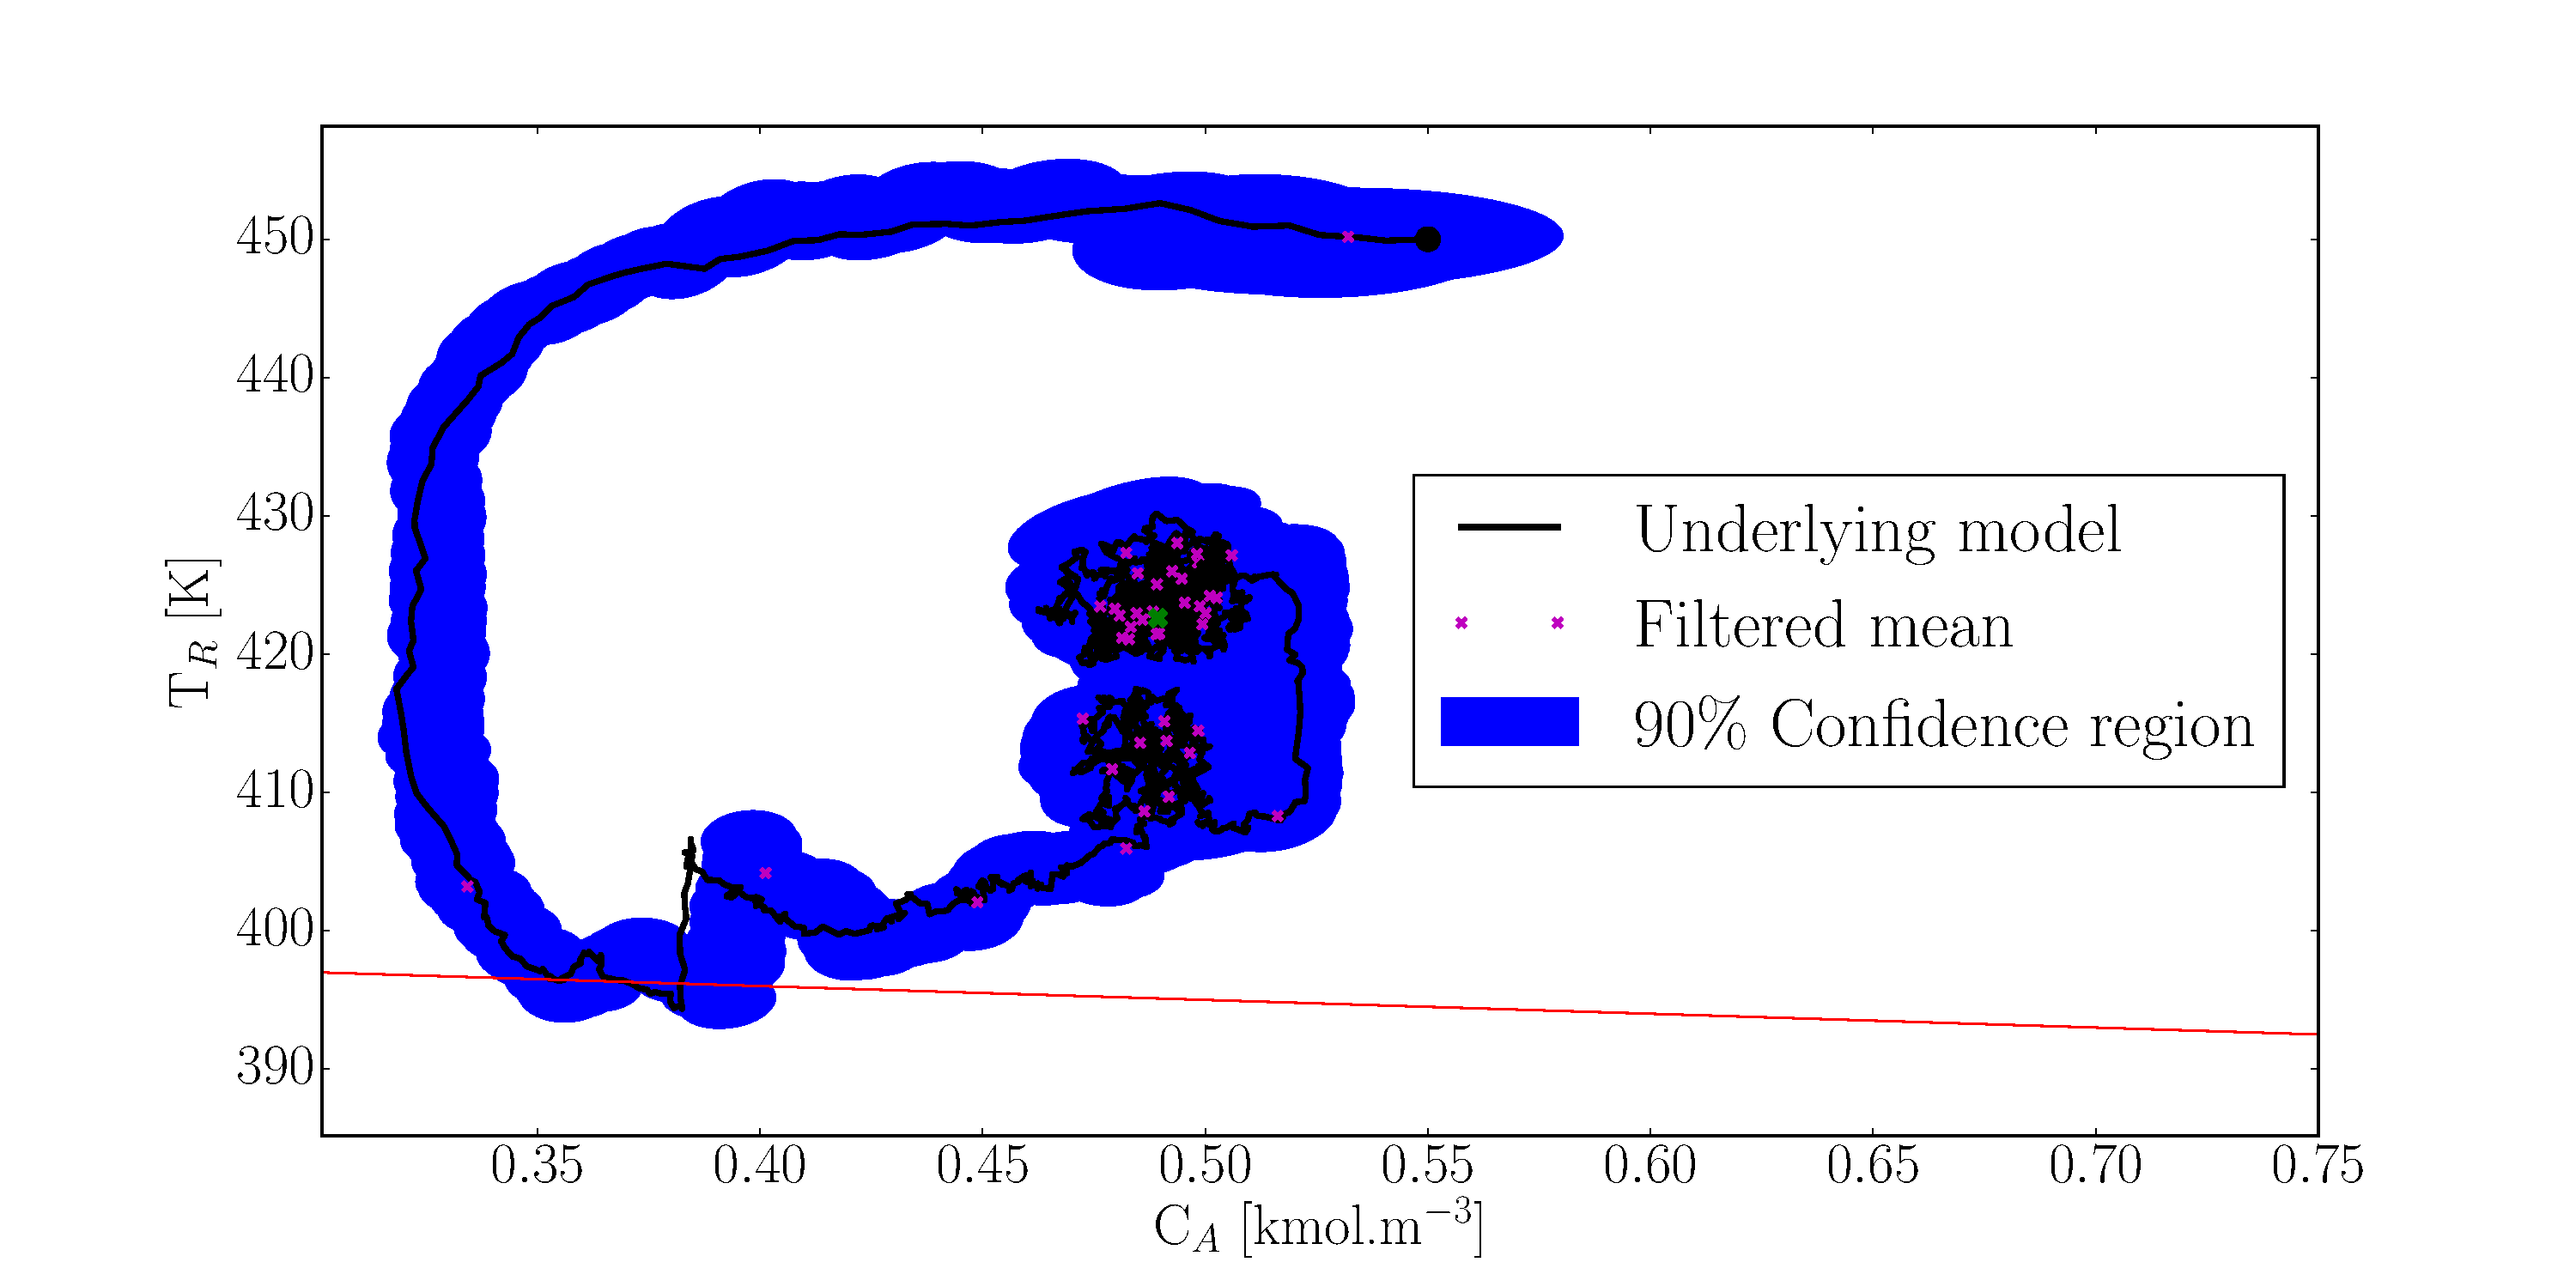
\includegraphics[scale=0.25]{spf_mpc_state.pdf}
\caption{State space trajectory of the expected value constrained stochastic MPC using the Switching Controller Algorithm.}
\label{fig_spf_mpc_state}
\end{figure}
Clearly there is a constraint violation - similar to that found in Chapter \ref{sec_lin_sys_cont} and \ref{sec_nonlinear_control}. By extending the MPC problem of (\ref{eq_spf_mpc_expected}) to the chance constrained (\ref{eq_spf_mpc_chance}) we attempt to ensure that the constraint is not violated. 
\begin{equation}
\begin{aligned}
&\underset{\mathbf{u}}{\text{min }} \mathbb{E}\left[ \frac{1}{2}\sum_{k=0}^{N-1} \left( x_k^TQx_k + u_k^TRu_k \right) + \frac{1}{2}x_N^TP_fx_N \right] \\
& \text{subject to } x_{t+1}=A_ix_t+B_iu_t + w_t~\text{(Latent)} \\
& \text{and } y_{t}= Cx_t + v_t \text{ (Observed)}\\
& \text{and } \mathbb{E}[\begin{pmatrix}
10 \\ 1
\end{pmatrix}^Tx_t + 400] \geq 0 ~\forall ~t=1,...,N \\
& \text{and } \text{Pr}(\begin{pmatrix}
10 \\ 1
\end{pmatrix}^T x_t + 400 \geq 0) \geq 0.99 ~\forall ~t=1,...,N\\
& \text{and } |u_t| \leq 15000 ~\forall ~t=0,...,N-1\\
\end{aligned}
\label{eq_spf_mpc_chance}
\end{equation} 
The same Switching Controller Algorithm, as discussed previously, is implemented. We have used the 99\% chance constraint to highlight the effectiveness of the method compared to the expected value version. 

In Figure \ref{fig_spf_mpc_track2} we see that the switching chance constrained MPC successfully tracks the set point.
\begin{figure}[H] 
\centering
\includegraphics[scale=0.25]{spf_mpc_track2.pdf}
\caption{The Switching MPC Controller Algorithm applied to the CSTR with catalyst which denatures at 100 minutes. The chance constrained MPC was used.}
\label{fig_spf_mpc_track2}
\end{figure}
The average concentration error is 2.97\% and the average controller input is 170 kJ/min. In Figure \ref{fig_spf_mpc_switch2} we see the familiar model switching diagram. Clearly the controller successfully isolates when the fault occurs.
\begin{figure}[H] 
\centering
\includegraphics[scale=0.25]{spf_mpc_switch2.pdf}
\caption{Most likely model identified using the Switching Particle Filter within the context of the chance constrained Switching MPC Controller Algorithm.}
\label{fig_spf_mpc_switch2}
\end{figure}
Finally, in Figure \ref{fig_spf_mpc_state2} we see that the constraint is not violated.
\begin{figure}[H] 
\centering
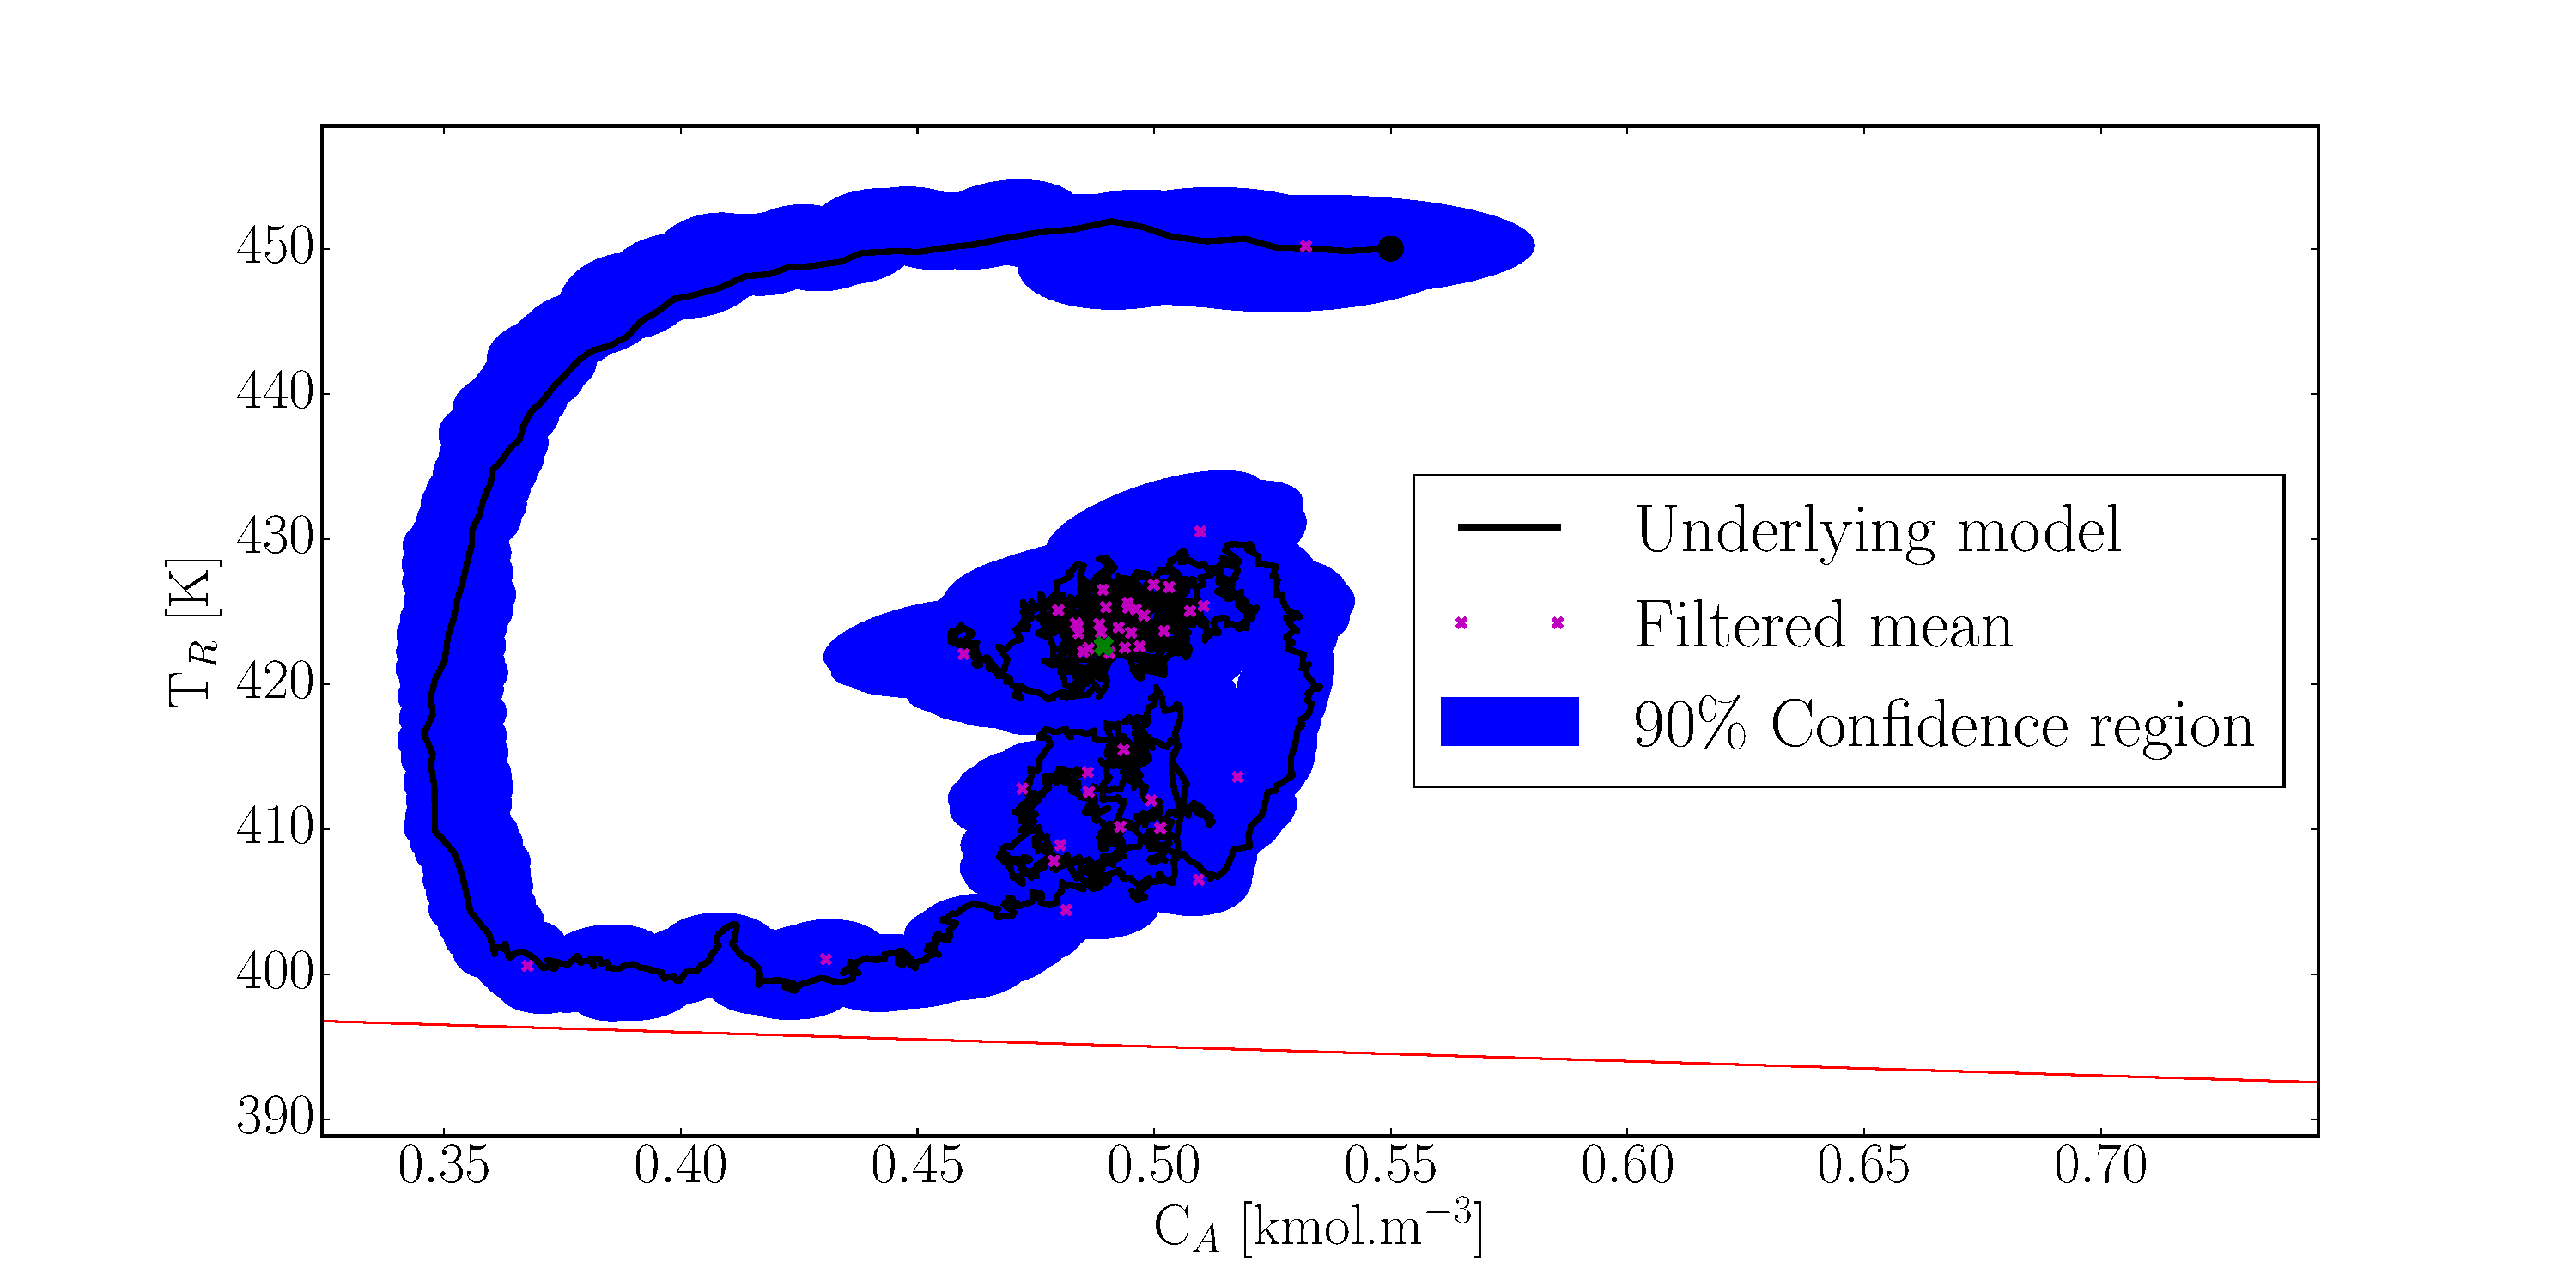
\includegraphics[scale=0.25]{spf_mpc_state2.pdf}
\caption{State space trajectory of the chance constrained stochastic MPC using the Switching Controller Algorithm.}
\label{fig_spf_mpc_state2}
\end{figure}
Since Figure \ref{fig_spf_mpc_state2} only illustrates that the constraint is not violated for a single run we again use a Monte-Carlo technique to justify the assertion that, for this example, the stochastic controller can successfully reduce the constraint violation probability. By simulating 100 runs it was found that the expected value stochastic MPC violated the constraint 156.9 times per run of 300 minutes. The chance constrained stochastic MPC violated the constraint 14.8 times per run of the same length. If the robustness of the Switching Controller can be improved there is significant upside to its implementation.

\section{Conclusion}
In this section we implemented the Switching Controller Algorithm using the Switching Particle Filter. Both the LQG and stochastic MPC were used in conjunction with the Switching Particle Filter. While the controllers successfully regulated the system the controller/filter combination was not robust against switching noise. Since this noise has the potential to destabilise control more research needs to be done to investigate effective methods to assure stability. The Augmented Switching Filter Model discussed in Chapter \ref{sec_rbpf_control} (for the linear ``Kalman" case) could be a potential candidate. While stability issues plagued the implementation of the system, the fault detection and superior state estimation ability of the Switching Particle Filter was found to be useful.


\begin{figure}[H] 
\centering
\begin{tikzpicture}

  % Define nodes
  \node[obs] (ya) {$y_{0}$};
  \node[obs, right=of ya] (yb) {$y_{1}$};
  \node[obs, right=of yb] (yc) {$y_{2}$};
  \node[latent, above=of ya]  (xa) {$x_{0}$};
  \node[latent, above=of yb, right=of xa]  (xb) {$x_{1}$};
  \node[latent, above=of yc, right=of xb]  (xc) {$x_{2}$};
  \node[det, below=of xa, xshift=0.7cm, yshift=0.9cm] (da) {$u_{0}$};
  \node[det, below=of xb, xshift=0.7cm, yshift=0.9cm] (db) {$u_{1}$};
  \node[latent, above=of xa, yshift=1.1cm] (sa) {$s_{0}$};
  \node[latent, above=of xb, yshift=1.1cm] (sb) {$s_{1}$};
  \node[latent, above=of xc, yshift=1.1cm] (sc) {$s_{2}$};
  
  % Connect the nodes
  \edge {da} {xb};
  \edge {db} {xc};
  \edge {xa} {ya};
  \edge {xb} {yb};
  \edge {xc} {yc};
  \edge {xa} {xb};
  \edge {xb} {xc};
  \edge {sa} {sb};
  \edge {sb} {sc};
  \edge {sa} {xa};
  \edge {sb} {xb};
  \edge {sc} {xc};
  \edge {xa} {sb};
  \edge {xb} {sc};
    
\end{tikzpicture}
\caption{Augmented Switching Kalman filter graphical model.}
\label{fig_gm_augmented}
\end{figure}
Using this model it is possible to specify the effect the state variables $(x_0,x_1,...)$ have on the switching variables $(s_0, s_1,...)$. Plausibly this could ameliorate the problem however, since this would require that we modify the graphical model we leave this for future work.  
